%2.4
\section{Absolutbetrag und reelle Lösungen von Gleichungen}

Der (Absolut)-Betrag ist die folgende Funktion:\\
\begin{center}
	$|\cdot|:\mathbb{R}\longmapsto [o,\infty[$\;\;  mit $ |x| =     \left\{ \begin{array}{rcl}
		x & \mbox{für} & x\geq0\\
		-x & \mbox{für} & x< 0 \;\;\;\;\;\;\;\; \text{(II.5) }\\
		
	\end{array}\right.$
\end{center}
\begin{center}
	\fbox{\parbox  {60mm} {
			\begin{center}
				Mit den Eigenschaften:\\
			\end{center}
			\begin{align*}
				&|x\cdot y|=|x|\cdot|y|\\
				&\text{\tiny Dreiecksungleichung: }\\
				&|x+y|\leq |x|+|y|
			\end{align*}
	}}
\end{center}
Beispiel:\\
\textbullet\;\;$|-7|=-(-7) =7 $ \tiny{(in Funktion (II.5) einsetzen)}\normalsize \\
\textbullet \;\;$|7|=7$\\
\textbullet \;\;$ x<2:|x+2|=-(x+2) $\\

Funktion: $ f(x)=|x| $\vspace*{2mm}\\
\begin{center}
	
	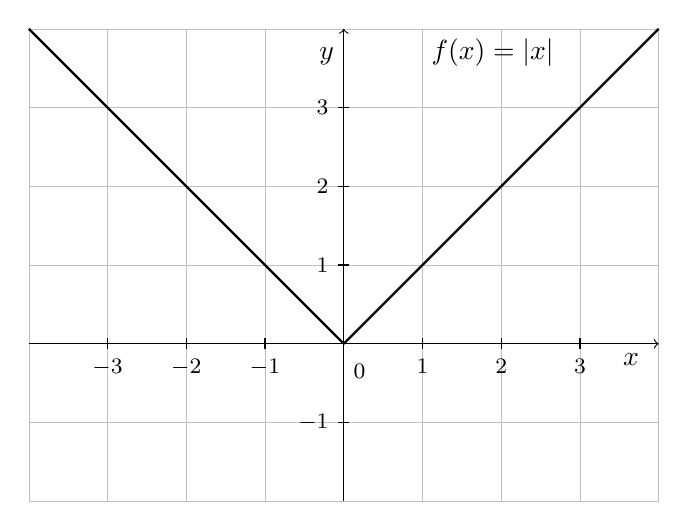
\begin{tikzpicture}
		
		% Gitternetzlinien
		\draw[xstep=1cm, ystep=1cm, very thin, color=lightgray] (-4,4) grid (4,-2);
		% x-Achse
		\draw[->] (-4,0) -- (4,0) node[below,xshift=-1em] {$x$}; 
		%Zahlen auf x-Achse
		\foreach \x in {-3,...,-1}
		\draw[shift={(\x,0)},color=black] (0pt,2pt) -- (0pt,-2pt) node[below] {\footnotesize $\x$};
		\foreach \x in {1,...,3}
		\draw[shift={(\x,0)},color=black] (0pt,2pt) -- (0pt,-2pt) node[below] {\footnotesize $\x$};
		% y-Achse 
		\draw[->] (0,-2) -- (0,4) node[left,yshift=-1em] {$y$};%node[above left]
		%Zahlen auf y-Achse
		\foreach \y in {-1,...,-1}
		\draw[shift={(0,\y)},color=black] (2pt,0pt) -- (-2pt,0pt) node[left] {\footnotesize $\y$};
		\foreach \y in {1,...,3}
		\draw[shift={(0,\y)},color=black] (2pt,0pt) -- (-2pt,0pt) node[left] {\footnotesize $\y$};
		%Ursprung
		\draw[color=black] (0pt,-10pt) node[right] {\footnotesize $0$};
		
		\draw[thick,color=black] plot[samples=200, domain=0:4] 
		(\x,{\x}) node[below, xshift=-6em] {$f(x)=|x|$};
		
		\draw[thick,color=black] plot[samples=200, domain=-4:0] 
		(\x,{-\x}) node[below, xshift=1em]{};
		
		
		
	\end{tikzpicture}\vspace*{4mm}\\
\end{center}
\newpage
\noindent
Löse folgende reelle Gleichung:\\
\begin{center}
	$ |x+2|-|x-2|=1 $ mit $ x \in \mathbb{R} $
\end{center}
Es muß eine Fallunterscheidung durchgeführt werden und zwar da, wo sich die Vorzeichen ändern.\\
Die Vorzeichen ändern sich bei -2 und +2.\\
Am Zahlenstrahl hat man dann 3 Fälle.\vspace*{2mm}
\\
\begin{tikzpicture}
	%\draw[->,>=stealth] (0,0)--++(-0.5,-0.5)--++(0.5,0)--++(-0.5,-0.5);
	
	\node at (2,0) [red,rotate=0] {$]$};
	\node at (1.8,-0.6) [black,rotate=0] {$-2$};
	\draw [red](0,0) -- (2,0) ;
	\draw [blue](2,0) -- (4,0) ;
	\node at (4,0) [green,rotate=0] {$[$};
	\draw [->,green](4,0) -- (6,0) ;
	\node at (4,-0.6) [black,rotate=0] {$2$};
\end{tikzpicture}\\
1.Fall: $ \textcolor{red}{x\leq2} $\\
2.Fall: $\textcolor{blue}{-2<x<2 } $\\
3.Fall: $ \textcolor{green}{x\geq 2} $\vspace*{2mm}\\
\underline{1.Fall:}\\
Für $x\leq-2  $ gilt:\\
\begin{align*}
	-(x+2)-(-(x-2))=-x-2+x-2=-4=1_{ \;\;\tikz \draw[->,>=stealth] (0,0)--++(-0.2,-0.2)--++(0.2,0)--++(-0.2,-0.2);}
\end{align*}
Für $ x\leq-2 $ gibt es keine Lösung!\vspace*{2mm}\\
\underline{2.Fall:}\\
Für $ -2<x<2 $ gilt:\\
\begin{align*}
	x+2-(-(x-2))=x+2+x-2=2x=1
\end{align*}
d.h. $ x=\frac{1}{2} $ ist eine Lösung.\vspace*{2mm}\\
\underline{3.Fall:}\\
$ 2\leq x $\\
\begin{align*}
	x+2-(x-2)=4=1_{ \;\;\tikz \draw[->,>=stealth] (0,0)--++(-0.2,-0.2)--++(0.2,0)--++(-0.2,-0.2);}
\end{align*}
Für $ 2\leq x $ gibt es keine Lösung!\\
\\
Fazit: Einzige Lösung ist $ x=\frac{1}{2} $.\\
\subsection{Aufgabe 1 zum Thema reelle Lösungen von Gleichungen}

Bestimme alle reellen Lösungen dieser Gleichung:\\
\begin{align*}
	\big||3x|-|-5|\big|=2
\end{align*}
Die Gleichung ist äquilalent zu:\\
\begin{align*}
	\big||3x|-|-5|\big|=2\Leftrightarrow\big||3x|-5\big|=2
\end{align*}
\newpage
\noindent
\underline{1.Fall:}\\
$ x\geq 0:\big||3x|-|-5|\big|=|3x-5| $ \\
\begin{quote}
	\underline{1.1Fall:}\\
	$x\geq \frac{5}{3}:|3x-5|=3x-5=2\Leftrightarrow 3x=7\Leftrightarrow x=\frac{7}{3}$\\
	\underline{1.2Fall:}\\
	$0<x<\frac{5}{3}:|3x-5|=-(3x-5)=-3x+5=2\Leftrightarrow -3x=-3\Leftrightarrow x=1$\\
\end{quote}
\underline{2.Fall:}\\
$x<0:\big||3x|-5\big|=|-3x-5|=|-1(3x+5)|=|(-1)||3x+5|=|3x+5|=2$\\
\begin{quote}
	\underline{2.1Fall:}\\
	$x<-\frac{5}{3}:|3x+5|=-(3x+5) =-3x-5=2\Leftrightarrow-3x=7\Leftrightarrow x=-\frac{7}{3} $\\
	\underline{2.2Fall:}\\
	$0\geq x\geq -\frac{5}{3} : |3x+5|=3x+5=2\Leftrightarrow 3x=-3\Leftrightarrow x=-1 $\\
\end{quote}
Fazit: $x_1=\frac{7}{3},\; x_2=1,\; x_3=-\frac{7}{3},\; x_4=-1$ lösen die Gleichung.\\

\subsection{Aufgabe 2 zum Thema reelle Lösungen von Gleichungen}

Bestimme alle reellen Lösungen der folgenden Ungleichung:\\
\begin{align*}
	x^3+11x<6x^2+6
\end{align*}
Zuerst Gleichung umstellen:\
\begin{align*}
	\Leftrightarrow \underbrace {x^3-6x+11x-6}_{=p(x)=(x-x_1)(x-x_2)(x-x_3)}<0
\end{align*}
NR:\\
Faktorisierung des Polynoms $ p(x) $\\
Durch hinschauen erhalten wir $ x_1=1 $ eine Nullstelle.\\
D.h. $ (x-x_1)=(x_1-1) $ teilt $ p(x) $\\
Mittels Polynomdivision ergibt sich:\\
\begin{center}
	\begin{tabular}[t]{lll}% l=linksbündig r=rechtsbündig
		&\;\;\;$(x^3-6x^2+11x-6)\div (x-1)=x^2-5x+6 $ \\
		&$-\underline{(x^3-\;\;x^2)} $  \\
		&\hspace{1.1cm}$ -5x^2+11x $\\
		&\hspace{0.6cm}$-\underline{(-5x^2+\;\;5x) }$\\
		&\hspace{2.8cm}$6x-6 $\\
		&\hspace{2.43cm}$\underline{-(6x-6)} $\\
		&\hspace{3.8cm}$0$\\
	\end{tabular} \\
\end{center}
\newpage
\noindent

$ p(x)=(x^2-5x+6)(x-1) $\\
Lösung der quatratischen Gleichung $ x^2-5x+6=0$.\\
\begin{align*}
	x^2-5x+6&=0\\
	x^2-5x+\frac{25}{4}-\frac{25}{4}+\frac{24}{4}&=0\\
	\bigg(x-\frac{5}{2}\bigg)^2-\frac{1}{4}&=0\\
	\bigg(x-\frac{5}{2}\bigg)^2&=\frac{1}{4}\\
	x-\frac{5}{2}&=\pm \sqrt{\frac{1}{4}}\\
	x_{2,3}&=\frac{5}{2}\pm \frac{1}{2}\\
	x_2&=3\\
	x_3&=2
\end{align*}
$ p(x)=(x-3)(x-2)(x-1) $\\
Jetzt kann man die Ungleichung durch die Faktorisierung leicht lösen:\\
\begin{align*}
	(x-3)(x-2)(x-1)<0
\end{align*}
Durch die Nullstellen $ x_1=1, x_2=3, x_3=2 $ bekommt man vier Fälle:\\
Am Zahlenstrahl hat man dann 4 Fälle.\vspace*{2mm}
\\
\begin{tikzpicture}
	%\draw[->,>=stealth] (0,0)--++(-0.5,-0.5)--++(0.5,0)--++(-0.5,-0.5);
	
	\node at (2,0) [red,rotate=0] {$][$};
	\node at (2,-0.6) [black,rotate=0] {$1$};
	\draw [red](0,0) -- (2,0) ;
	\draw [blue](2,0) -- (4,0) ;
	\node at (4,0) [green,rotate=0] {$][$};
	\draw [green](4,0) -- (6,0) ;
	\node at (4,-0.6) [black,rotate=0] {$2$};
	\draw [->,black](6,0) -- (8,0) ;
	\node at (6,-0.6) [black,rotate=0] {$3$};
	\node at (6,0) [black,rotate=0] {$][$};
\end{tikzpicture}\\
Bei $ x_1=1, x_2=3, x_3=2 $ wird das Polynom zu Null. Also keine Lösung, da Polynom $ <0 $ werden soll.\\
Für die 4 Fälle gilt dann:\\
\begin{center}
	\( \begin{array}{|l|c|c|c|c|}
		\hline       &(x-1)&(x-2)&(x-3)&p(x)\\
		\hline 1.Fall: x<1&-&-&-&-\\
		\hline 2.Fall: 1<x<2&+&-&-&+\\
		\hline 3.Fall: 2<x<3&+&+&-&-\\
		\hline 4.Fall: x>3&+&+&+&+\\
		\hline
	\end{array} \)
\end{center}
Fazit:\\
Bei $ x<1 $ und  $ 2<x<3 $ wird das Polynom negativ. Also ist die Lösung:\\
\begin{align*}
	x\in \;]-\infty,1[\;\; \cup \;\;]2,3[
\end{align*}



